\documentclass[11pt]{article}
\usepackage[utf8]{inputenc}
\usepackage[T1]{fontenc} % uses T1 fonts (better quality)
\usepackage{lmodern} % uses Latin Modern fonts
\usepackage[margin=1in]{geometry}
\usepackage[dvipsnames]{xcolor}
\usepackage{ragged2e}
\renewcommand{\baselinestretch}{1.15}
\usepackage{tikz}
\usetikzlibrary{automata,scopes,shapes,matrix,arrows,decorations.pathmorphing}
\tikzset{>={stealth}}
\usepackage{mathtools}
\usepackage{bm}
\usepackage{graphicx}
\usepackage{wrapfig}
\usepackage[makeroom]{cancel}
\definecolor{OuterBlue}{HTML}{1370AA}
\definecolor{InnerBlue}{HTML}{9BC4DD}
\usepackage{pdfpages}
\usepackage{amssymb}
\usepackage{rotating}
% \definecolor{CrispBlue}{HTML}{0176AE}
% \colorlet{answer}{CrispBlue}
% \renewenvironment{center}{\par\centering\color{answer}}
% \renewenvironment{align*}{\color{answer}}

\begin{document}
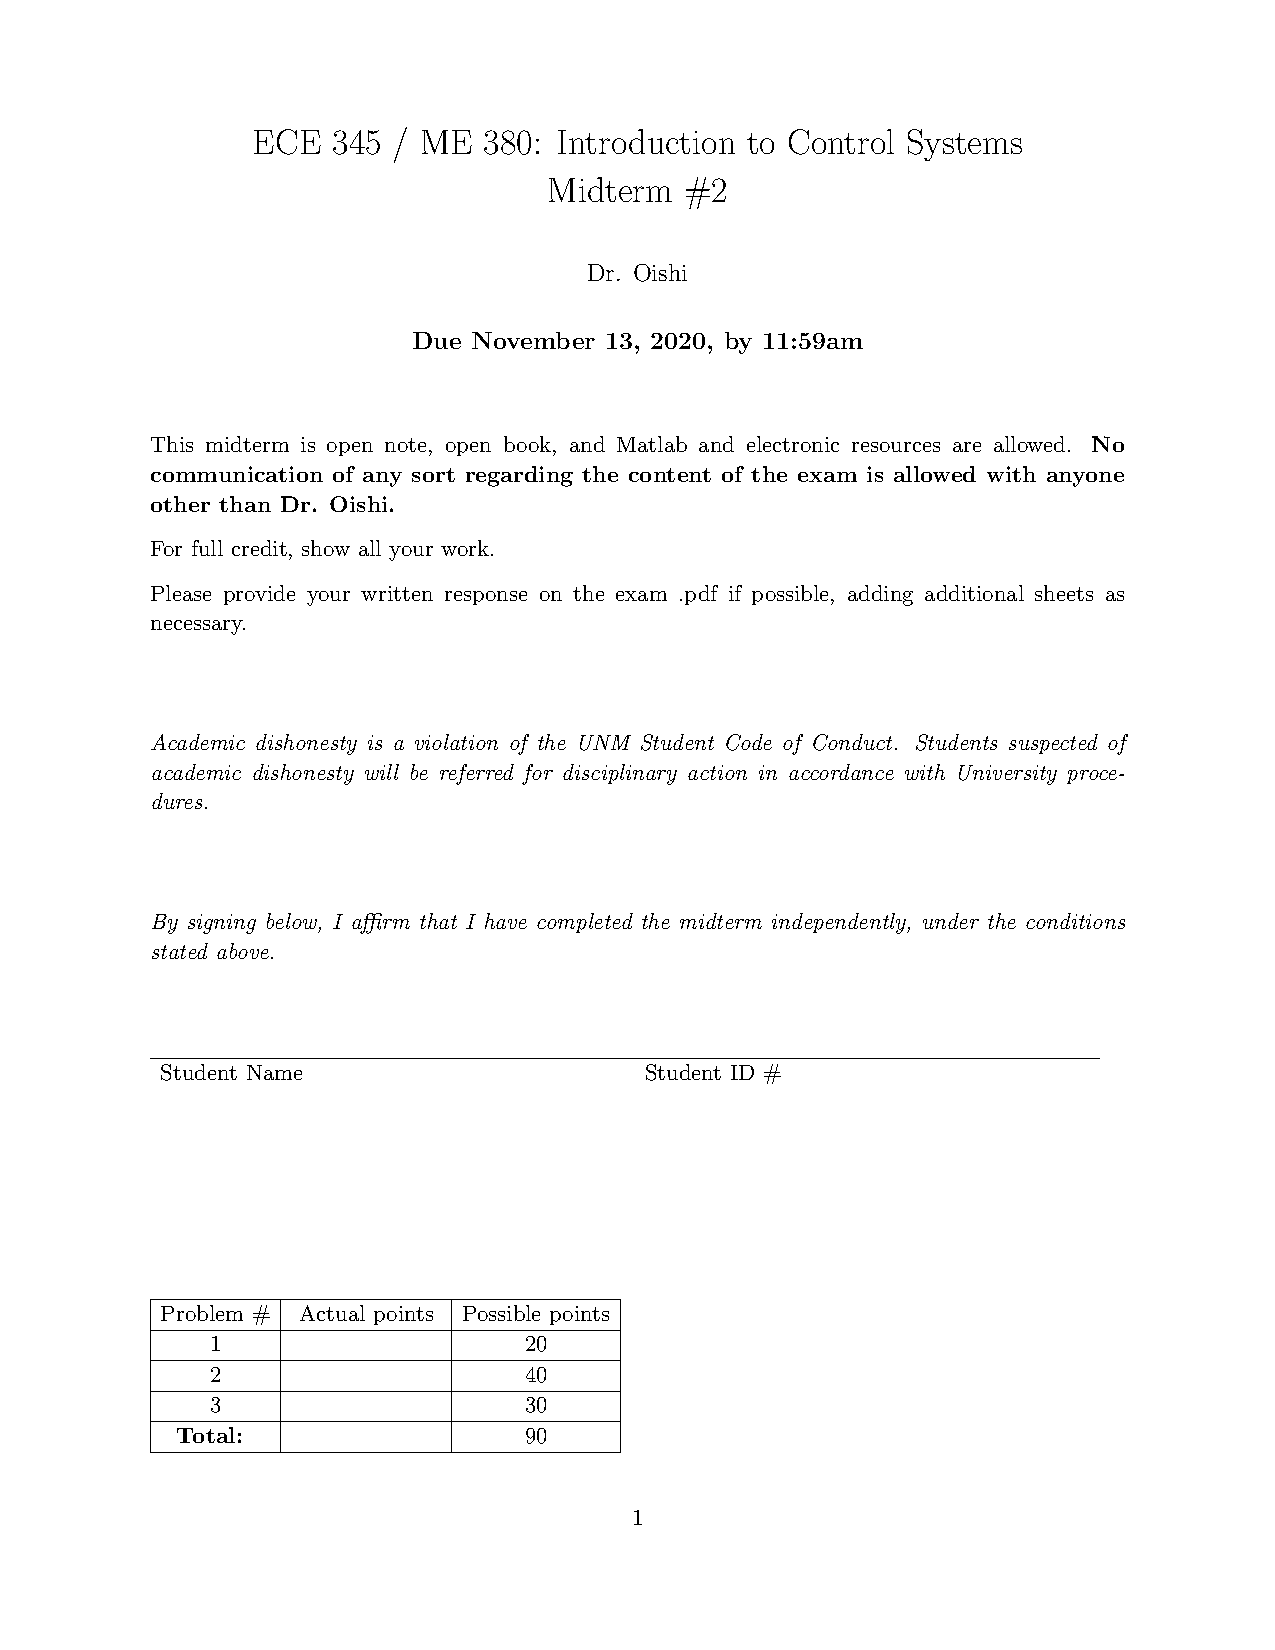
\includepdf[pages=1]{Midterm2(1).pdf}
\section{BIBO stability (20 points)}
Consider the transfer function \( G(s)=\displaystyle\frac{s}{(s+1)(s^2 + 3s + a)} \), where \(a\) is a real-valued number.
\begin{enumerate}
    \item (10 points) Use a Routh table to assess asymptotic stability of \( G(s)\). Which of the following is most correct?
    \begin{enumerate}
        \item The closed-loop system is unstable for \(a<-4\) since there are \textit{two} poles in the RHP.
        \item The closed-loop system is unstable for \(a>4\) since there are \textit{two} poles in the RHP.
        \item The closed-loop system is unstable for \(0>a>4\) since there is \textit{one} pole in the RHP.
        \item The closed-loop system is stable for \(a<0\) since there are \textit{no} poles in the RHP.
    \end{enumerate}\newpage
    Recall \( G(s)=\displaystyle\frac{s}{(s+1)(s^2 + 3s + a)} \).
    \item (10 points) Presume \(a= 2\). Which one of the following is correct?
    \begin{enumerate}
        \item Since \(G(s)\) is marginally stable, it is also BIBO stable.
        \item Since \(G(s)\) is BIBO stable, it is also asymptotically stable.
        \item Since \(G(s)\) is asymptotically stable, it is also BIBO stable.
        \item Since \(G(s)\) is asymptotically stable, there may be bounded input trajectories that generate unbounded output trajectories, hence more work is needed to assess BIBO stability.
        \item Since \(G(s)\) is asymptotically unstable, it is also BIBO unstable.
    \end{enumerate}
\end{enumerate}\newpage
\section{Precision welding (40 points)}
\begin{wrapfigure}[3]{r}{0.5\textwidth}
    \centering
    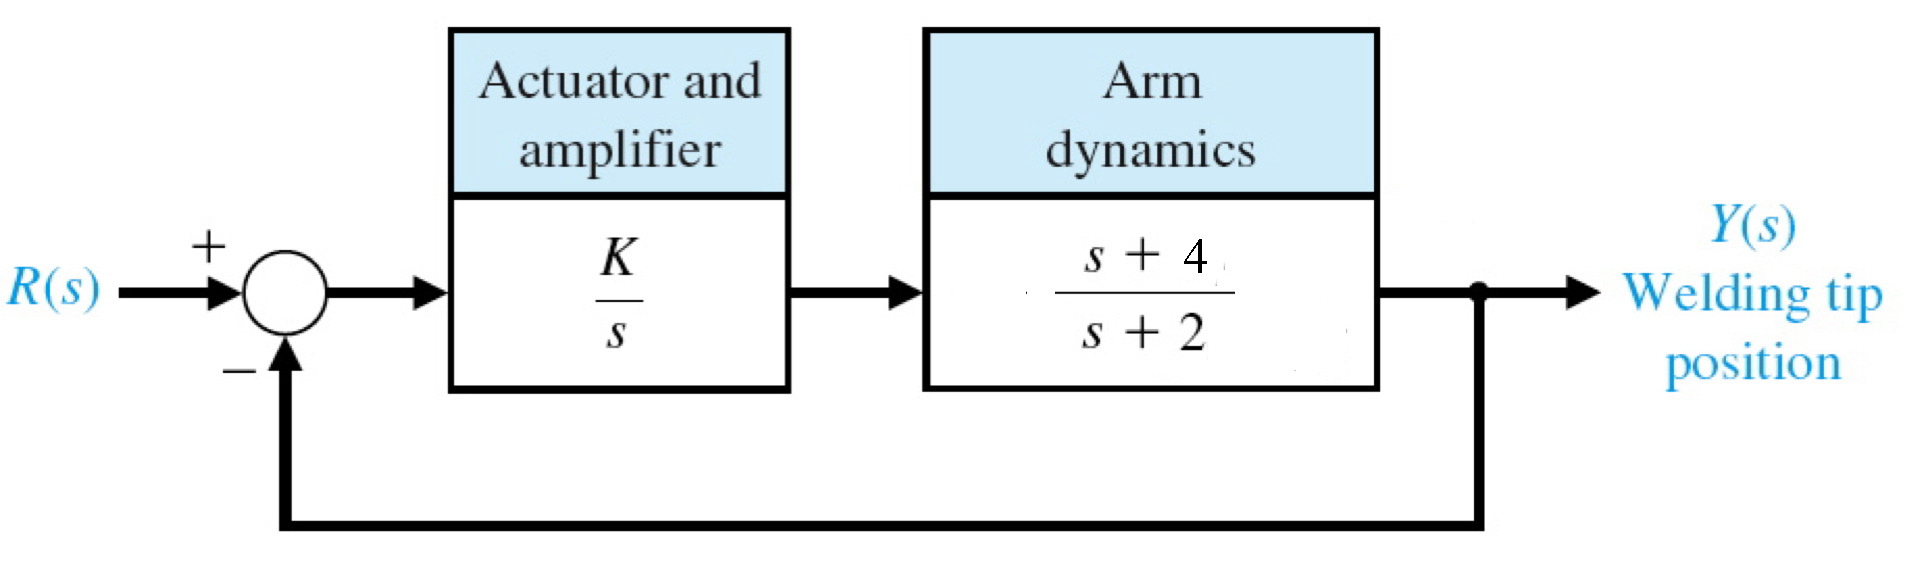
\includegraphics[width=0.5\textwidth]{Acr12457187579904187728.png}
\end{wrapfigure}
An automated welding machine must be precise and agile. Consider the welding system on the right.\vspace{3em}
    \begin{enumerate}
        \item (10 points) Consider the root locus plot of the system, shown below. Is it possible to find a gain \(K\) such that the poles of \(\frac{Y(s)}{R(s)}\) are located at \(4\pm 4j\)? In a single sentence, describe why or why not. \textit{You do not need to find the value of \(K\), if it is possible to do so.}
        \begin{figure}[h!]
            \centering
            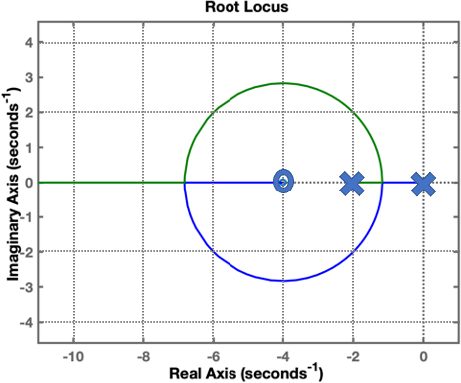
\includegraphics[width=0.55\textwidth]{Acr12457187579904-2994711.png}
        \end{figure}
        \item (10 points) Based on the root locus plot above, which one of the following is correct?
        \begin{enumerate}
            \item The open-loop system \(\frac{K(s+4)}{s(s+2)}\) is asymptotically stable for all \(K>0\) because all of the poles lie in the open left half plane for any \(K>0\).
            \item The closed-loop system \(\frac{Y(s)}{R(s)} \)is asymptotically stable for all \(K>0\) because all of the poles lie in the open left-half plane for any \(K>0\).
            \item The closed-loop system \(\frac{Y(s)}{R(s)} \) is marginally stable for all \(K>0\) because there is always a pole on the imaginary axis, and all other poles are in the open left half plane.
            \item The stability of the closed-loop system \(\frac{Y(s)}{R(s)} \) cannot be inferred from this plot.
        \end{enumerate}
        \item (10 points) Which one of the following describes the characteristic equation of the closed-loop system? \textit{Show your work for full credit.}
        % \begin{wrapfigure}[3]{r}{0.5\textwidth}
        %     \centering
        %     \includegraphics[width=0.5\textwidth]{}
        % \end{wrapfigure}

\end{enumerate}
\end{document}